% Russian language
\documentclass{article}
\usepackage[utf8]{inputenc}
\usepackage[russian]{babel}

% Math symbols
\usepackage{amssymb}
\usepackage{amsmath}

% Images inplace
\usepackage{float}
\usepackage{graphicx}

% Code blocks
\DeclareFixedFont{\ttb}{T1}{txtt}{bx}{n}{12} % for bold
\DeclareFixedFont{\ttm}{T1}{txtt}{m}{n}{12}  % for normal
\usepackage{color}
\definecolor{deepblue}{rgb}{0,0,0.5}
\definecolor{deepred}{rgb}{0.6,0,0}
\definecolor{deepgreen}{rgb}{0,0.5,0}
\usepackage{listings}
\newcommand\pythonstyle{\lstset{
language=Python,
basicstyle=\ttm,
morekeywords={self},              % Add keywords here
keywordstyle=\ttb\color{deepblue},
emph={MyClass,__init__},          % Custom highlighting
emphstyle=\ttb\color{deepred},    % Custom highlighting style
stringstyle=\color{deepgreen},
frame=tb,                         % Any extra options here
showstringspaces=false
}}
\lstnewenvironment{python}[1][]
{
\pythonstyle
\lstset{#1}
}
{}
\newcommand\pythonexternal[2][]{{
\pythonstyle
\lstinputlisting[#1]{#2}}}
\newcommand\pythoninline[1]{{\pythonstyle\lstinline!#1!}}
% Code blocks


\title{Лабораторная работа №}
\author{Ларин Егор. 4 группа 2 курс}

\begin{document}
\maketitle
\section*{Теория}
\subsection*{Корни многочлена Чебышева на отрезке $[a,b]$}

\begin{equation*}
x^{ch}_k = \frac{(a+b)}{2}  + \frac{(b-a)}{2} \cos \left( \frac{2k + 1}{2n+2}\pi \right ), a=-2,b=2
\end{equation*}
\subsection*{Равностоящие узлы}
\begin{equation*}
x_k = a + \frac{k(b-a)}{n}, a=-2,b=2
\end{equation*}
\subsection*{Интерполяционный многочлен Ньютона}
\begin{equation*}
    P_n(x) = f(x_0) + (x-x_0) f(x_0; x_1) + (x-x_0)(x-x_1)f(x_0;x1;x_2)+ \dots + (x-x_0)\dots(x-x_{n-1}) f(x_0; \dots x_n),
\end{equation*}
где $f(x_0;\dots;x_k)$ -- разделенная разность $k$-ого порядка.

\section*{Листинг кода}
Многочлен представлен матрицей размера $n+1 \times n$. Первый столбец содержит интерполяционные узлы.
Второй столбец содержит значения интерполируемой функции в узлах. Оставшиеся столбцы содержат разделенные разности соответствующих порядков.
\begin{python}
from math import exp, cos, pi
import matplotlib.pyplot as plt

a = -2
b =  2

f_1 = lambda x: exp(cos(x))
f_2 = lambda x: abs(x * abs(x) - 1)

x_ch = lambda k, n: (a+b)/2  + (b-a) / 2 * cos((2*k + 1)*pi / (2*n +2))
x_ = lambda i, n: a + i*(b-a)/n

def newton(x, y, n):
    xss = [x(i, n) for i in range(n)]
    yss = [y(xss[i]) for i in range(n)]
    coefficients = [xss, yss]
    for i in range(1, n):
        prev = coefficients[i]
        diff = []
        for j in range(0, n-i):
            d = (prev[j] - prev[j+1]) / (xss[j] - xss[j+i])
            diff.append(d)
        coefficients.append(diff)
    return coefficients

def calc(x, c):
    ans = 0
    factor = 1
    n = len(c[0])
    for i in range(n):
        ans = ans + c[i+1][0] * factor
        factor = factor * (x-c[0][i])
    return ans

def compare(f, n):
    c = newton(x_, f, n)
    c_ch = newton(x_ch, f, n)
    m = 100
    xss = [x_(i, m) for i in range(m)]
    print(n)
    print(f"Ordinary error: {max(f, c)}")
    print(f"Chebyshev error: {max(f, c_ch)}")
    print()

    plt.plot(
            xss, [calc(x,c) for x in xss], "b",
            xss, [calc(x,c_ch) for x in xss],  "r",
            xss, [f(x) for x in xss], "g",

            c_ch[0], [f(x) for x in c_ch[0]], "ro",
            c[0], [f(x) for x in c[0]], "bo")
    plt.show()

def max(f, c):
    n = 101
    m = abs(calc(x_(0, n), c)  - f(x_(0, n)))
    for i in range(n):
        temp = abs(calc(x_(i, n), c)  - f(x_(i, n)))
        if temp > m:
            m = temp
    return m

print("f_1")
for i in [5, 10, 15, 20]:
    compare(f_1, i)

print("f_2")
for i in [5, 10, 15, 20]:
    compare(f_2, i)
    

\end{python}

\section*{Результаты вычислительного эксперимента}
\begin{figure}[H]
\caption{}
\centering
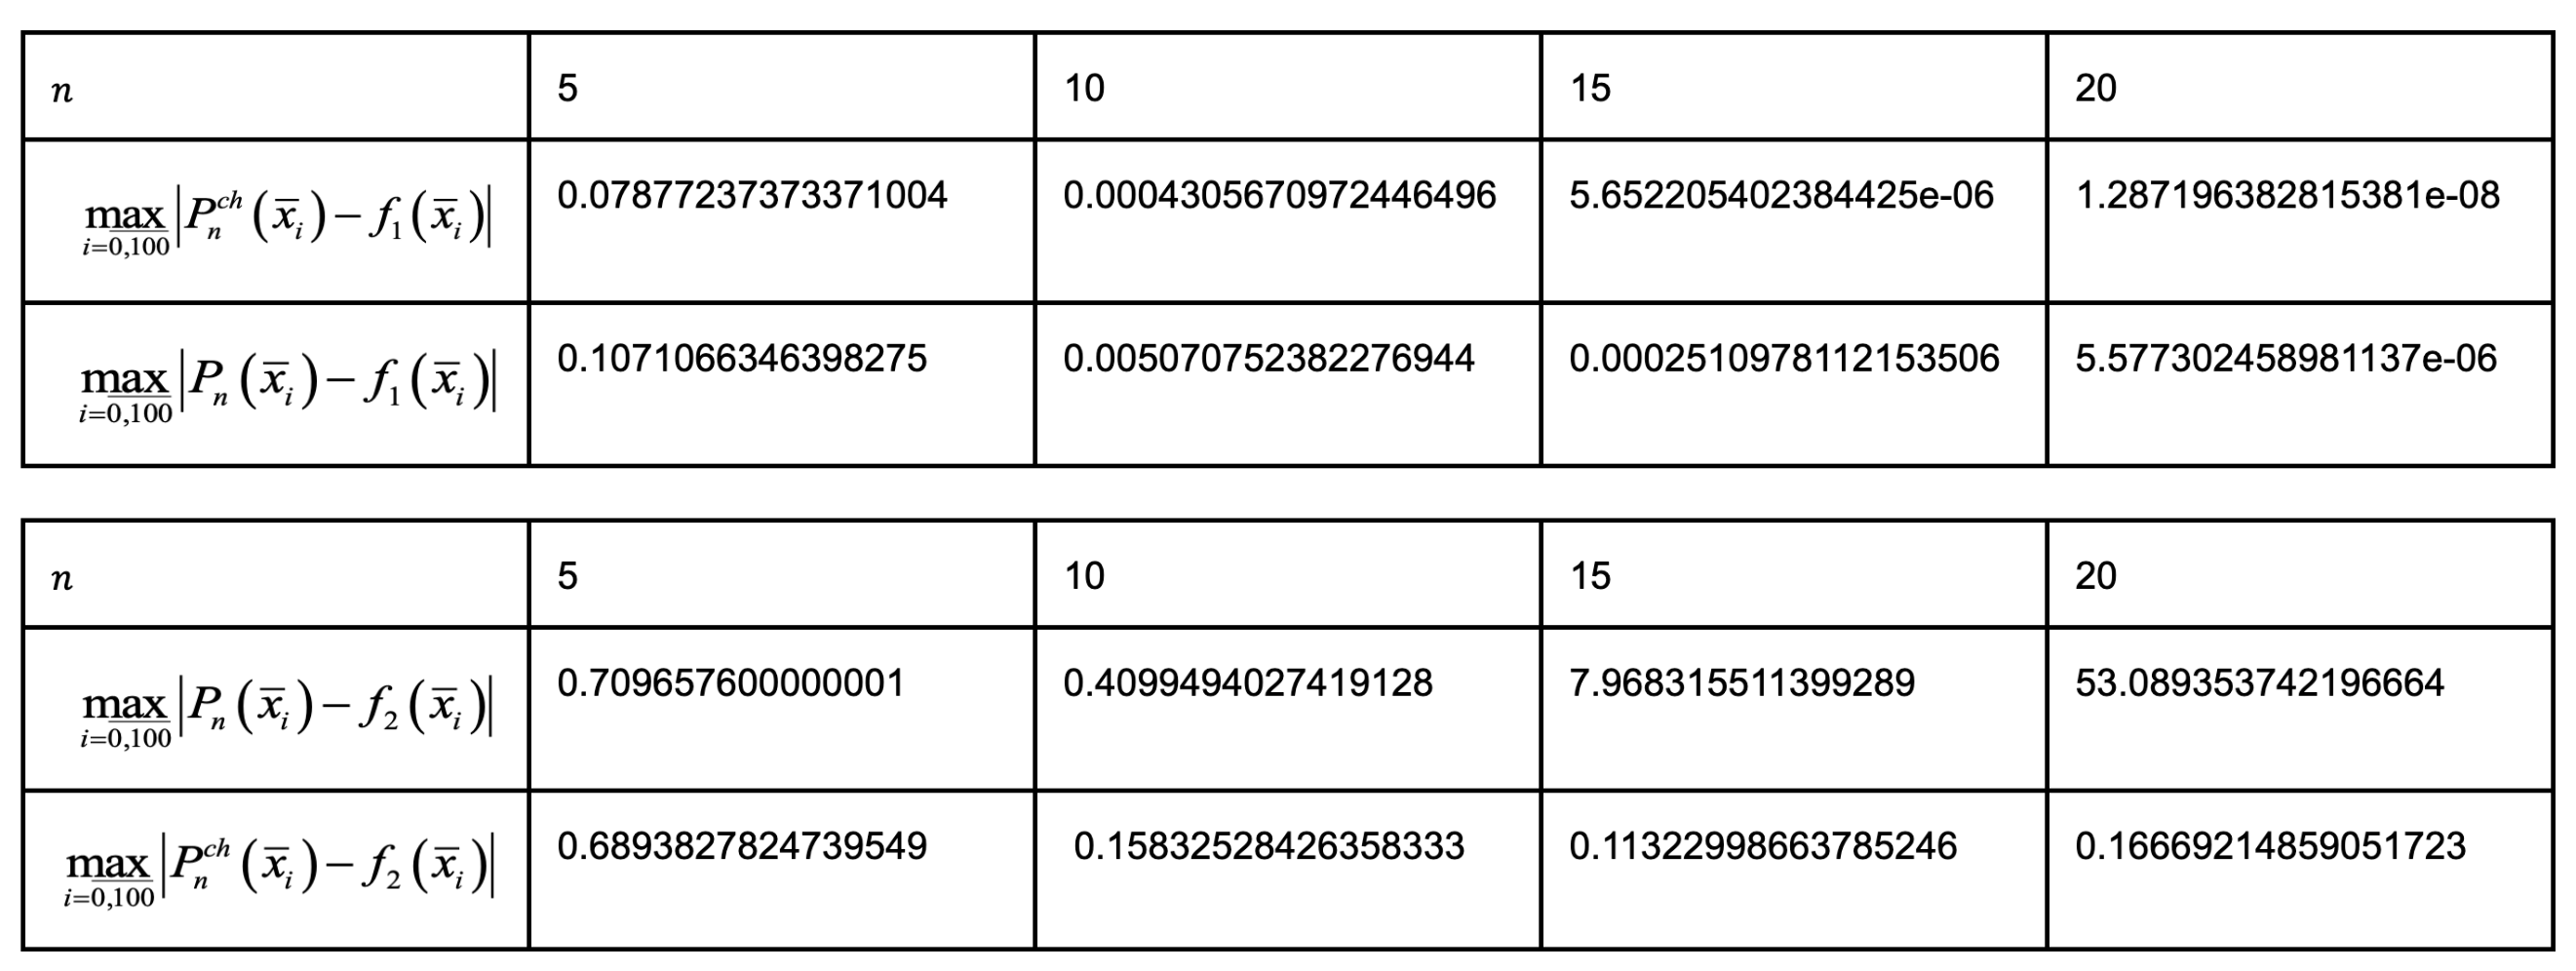
\includegraphics[width=0.9\textwidth]{table}
\end{figure}
\section*{Выводы}
Узлы Чебышева действительно являются оптимальными. При этом при интерполировании
функций, производная которых не является непрерывной, возникает значительная
ошибка, которая, справедливости ради, все еще меньше, чем при интерполировании
по равностоящим узлам.

\section*{Графики}
Зеленым обозначена исходная функция.
Красным обозначен график полинома интерполяции, полученный при использовании узлов Чебышева.
Зеленым обозначена исходная функция.
Синим обозначен график полинома интерполяции, полученный при использовании равностоящих узлов.
\subsection*{Графики для $f_1$}
\begin{figure}[H]
\caption{$n=5$}
\centering
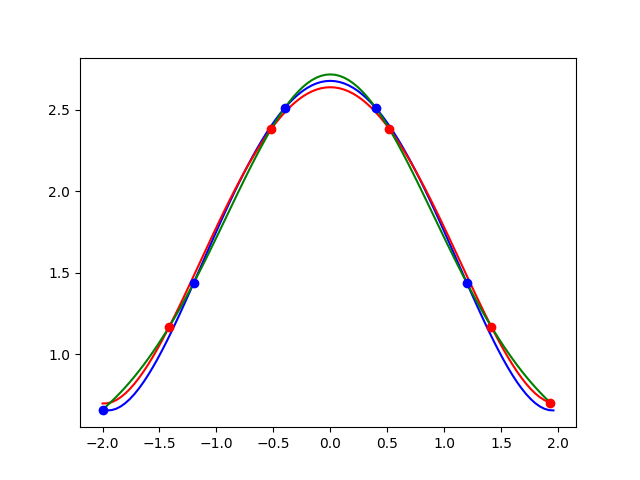
\includegraphics[width=0.9\textwidth]{f1_5}
\end{figure}
\begin{figure}[H]
\caption{$n=10$}
\centering
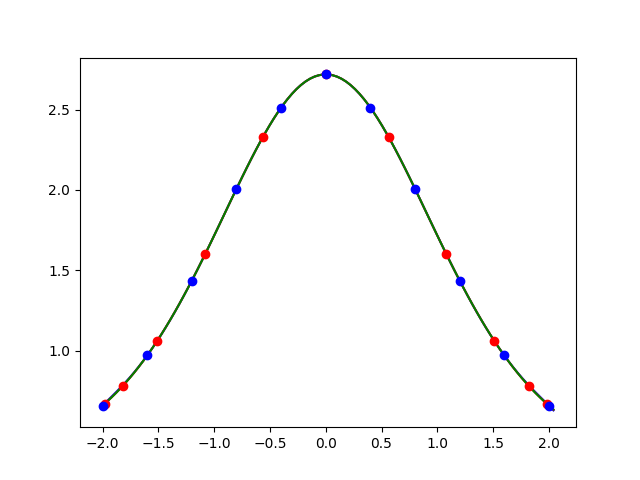
\includegraphics[width=0.9\textwidth]{f1_10.png}
\end{figure}
\begin{figure}[H]
\caption{$n=15$}
\centering
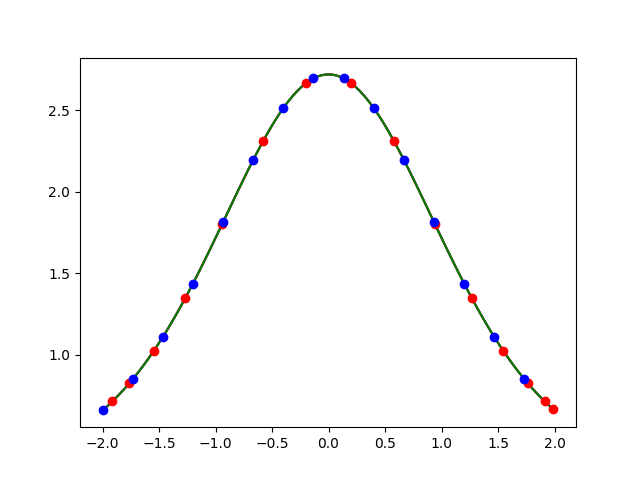
\includegraphics[width=0.9\textwidth]{f1_15}
\end{figure}
\begin{figure}[H]
\caption{$n=20$}
\centering
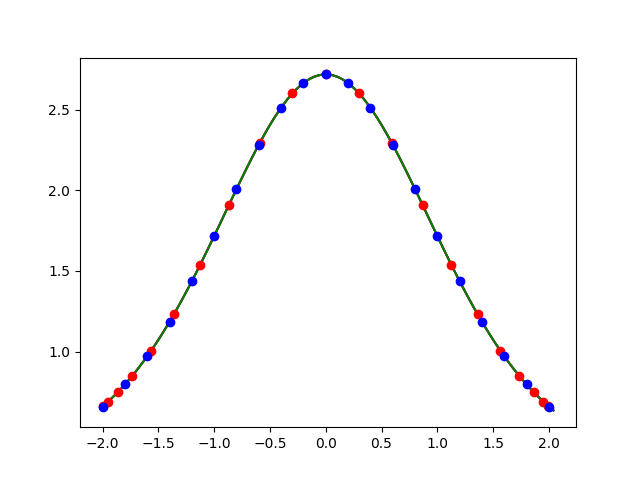
\includegraphics[width=0.9\textwidth]{f1_20}
\end{figure}

\subsection*{Графики для $f_2$}
\begin{figure}[H]
\caption{$n=5$}
\centering
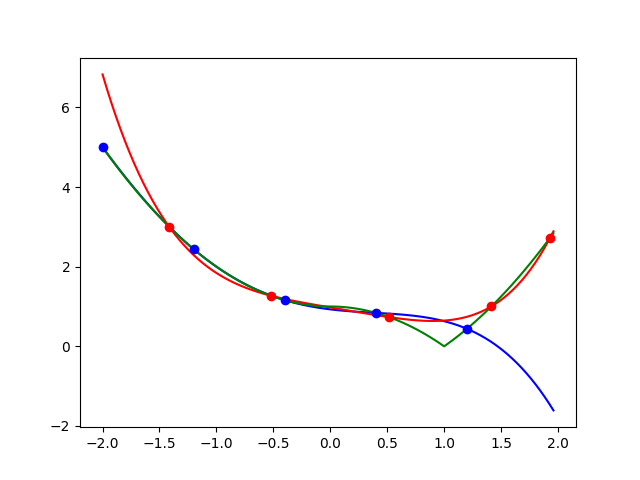
\includegraphics[width=0.9\textwidth]{f2_5}
\end{figure}
\begin{figure}[H]
\caption{$n=10$}
\centering
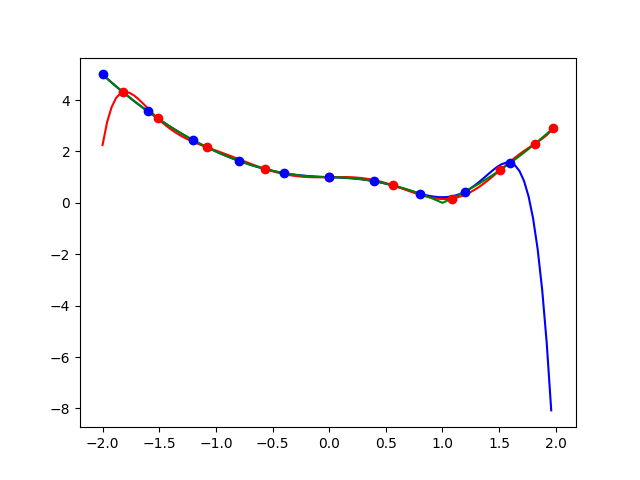
\includegraphics[width=0.9\textwidth]{f2_10.png}
\end{figure}
\begin{figure}[H]
\caption{$n=15$}
\centering
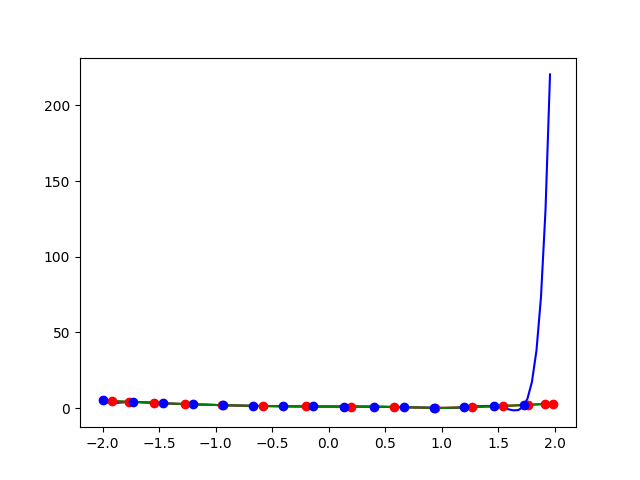
\includegraphics[width=0.9\textwidth]{f2_15}
\end{figure}
\begin{figure}[H]
\caption{$n=20$}
\centering
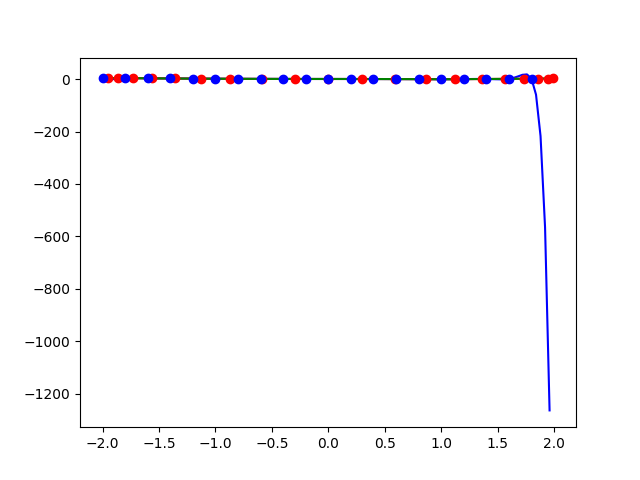
\includegraphics[width=0.9\textwidth]{f2_20}
\end{figure}
\end{document}

